\documentclass{beamer}

\usepackage[utf8]{inputenc}
\usepackage{default}
\usepackage{soul}
\makeatletter
\newcommand\SoulColor{%
  \let\set@color\beamerorig@set@color
  \let\reset@color\beamerorig@reset@color}
\makeatother

\begin{document}
\begin{frame}{A case for Keywords}
 \begin{itemize}
  \item A large number of false matches had no reference to the relation involved.
  \item Eg. No mention of Population in the following matches:
  \begin{itemize}
  \item The website of \SoulColor\hl{China's} Ministry of Defense (MOD) has attracted around \SoulColor\hl{1.25} billion visits in the three months since its opening, with the United States topping the source countries for foreign visits, website editor-in-chief Ji Guilin said.
  \item Insulza, for his part, said the Organization of American States expects to raise \SoulColor\hl{10 million} dollars for \SoulColor\hl{Haiti's} recovery.
  \item Koloini and others brought 10 million euros, probably \SoulColor\hl{15 million}, back from \SoulColor\hl{Iraq} at the time, Falter quoted from the diary.
 \end{itemize}
\item No reference to Co2 emission:
 \begin{itemize}
 \item \SoulColor\hl{China's} iron ore imports surged 41.6 percent to \SoulColor\hl{627.8 million tonnes} in 2009, with the value falling 17.4 percent as prices were hit by the global downturn, customs data shows.
 \end{itemize}
 \end{itemize}

\end{frame}

\begin{frame}{A case for Keywords}
 \begin{exampleblock}{Good News}
  Sentences expressing a numerical relation can be expected to have keywords that denote the relation
 \end{exampleblock}

 \begin{itemize}
  \item Take all the labeled sentences, prune out sentences that don't have atleast one of the relevant keywords
 \end{itemize}
 
 \begin{tabular}{|l|l|}
  \hline
  Internet User \% & "Internet" \\
Land Area & "area", "land", "land area" \\
Population &"Population" \\
Diesel & "diesel" \\
GDP &"Gross domestic", "GDP" \\
CO2 &"Carbon", "Carbon Emission", "CO2" \\
Inflation & "Inflation", "Price Rise" \\
FDI & "Foreign", "FDI" \\
Goods Export & "goods" \\
Life Expectancy & "life", "life expectancy" \\
Electricity Production & "Electricity" \\
 \hline
 \end{tabular}
\end{frame}

\begin{frame}{A case for Keywords}
\begin{itemize}
  \item Numbers are the second entity in our setup (Relation(Country, Number))
  \item Unlike real world entities, numbers don't have an identity of their own, sentences should have words (keywords!) indicating what the number stands for
  \item Manual inspection of 400 sentences pruned out after applying keyword based filter backs this conjecture, not even one false negative
  \item The keywords are created manually, can this process be automated?
\end{itemize}
\end{frame}

\begin{frame}
\begin{center}
 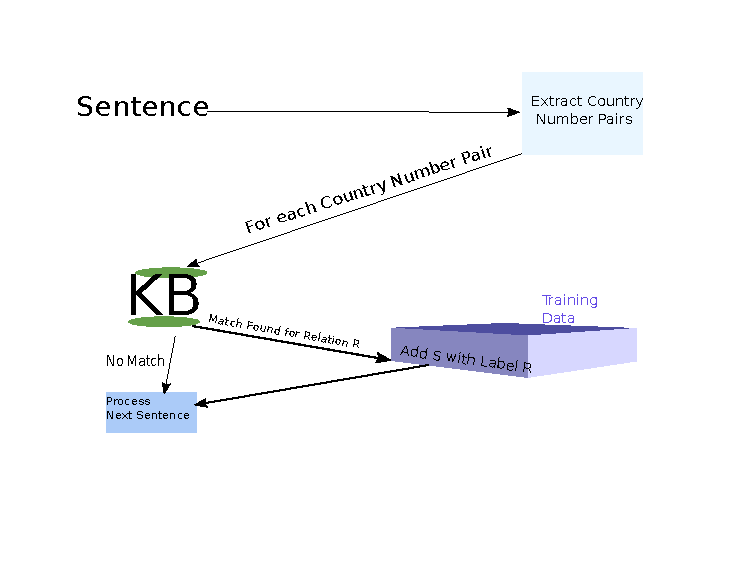
\includegraphics{./imgs/simple.pdf}
 % simple.eps: 0x0 pixel, 300dpi, 0.00x0.00 cm, bb=0 -1 348 200
\end{center}

\end{frame}

\end{document}
